\documentclass[a4paper, 11pt, final, garamond]{book}
\usepackage{cours-preambule}

\makeatletter
\renewcommand{\@chapapp}{Chimie -- chapitre}
\makeatother

\hfuzz=5.002pt

% \toggletrue{student}
% \toggletrue{corrige}
% \renewcommand{\mycol}{black}
\renewcommand{\mycol}{gray}

\begin{document}
\setcounter{chapter}{6}

\settype{enon}
\settype{solu_prof}
\settype{solu_stud}

\chapter{\cswitch{Correction du TD}{TD~: Diagrammes $E-\pH$}}

\resetQ
\section{Diagramme $E-\pH$ de l'argent}
\enonce{%
	\noindent
	\begin{minipage}[c]{.55\linewidth}
		On donne ci-dessous le diagramme potentiel-pH de l'argent, établi à
		\SI{25}{\degreeCelsius} en tenant compte des espèces $\ce{Ag_{\sol}}$,
		$\ce{{Ag_2O}_{\sol}}$ et $\ce{{Ag}^+_{\aqu}}$, et pour une
		concentration de tracé en ions argent égale à $c_t = \SI{0.1}{mol.L^{-1}}$.
		\bigbreak
		On superpose au diagramme les droites relatives aux couples
		$\ce{H_2O_{\liq}/{H_2}_{\gaz}}$ et $\ce{{O_2}_{\gaz}/H_2O_{\liq}}$,
		tracées pour $p_{t} = \SI{1}{bar}$. On donne $E^\circ (\ce{Ag^+/Ag}) =
			\SI{0.80}{V}$ et $E^\circ (\ce{Ag_2O/Ag}) = \SI{1.17}{V}$.
	\end{minipage}
	\hfill
	\begin{minipage}[c]{.40\linewidth}
		\vspace{0pt}
		\begin{center}
			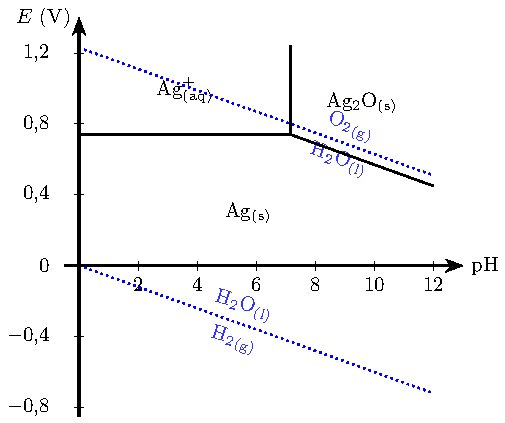
\includegraphics[width=\linewidth]{eph_ag-eau}
		\end{center}
	\end{minipage}
}%
\QR{%
	Établir l'équation de la frontière relative au couple $\ce{Ag^+/Ag}$.
}{%
	\leavevmode\vspace*{-15pt}\relax
	\begin{gather*}
		\ce{
		Ag_{\sol}
			=
			{Ag}^+_{\aqu} + e^-
		}
		\\\Ra
		E = E^\circ (\ce{Ag^{+}/Ag}) + \num{0.06}\log \frac{[\ce{Ag^+}]}{c^\circ}
		\\\beforetext{$[\ce{Ag^+}]\ind{front} = c_t \Ra$}
		\boxed{E\ind{front} = E^\circ(\ce{Ag^{+}/Ag}) - \num{0.06}}
		\Ra
		\xul{E\ind{front} = \SI{0.74}{V}}
	\end{gather*}
}%
\QR{%
	Déterminer la pente de la frontière relative au couple $\ce{Ag_2O/Ag}$.
}{%
	\leavevmode\vspace*{-15pt}\relax
	\begin{gather*}
		\ce{2Ag_{\sol} + H_2O_{\liq} = Ag_2O_{\sol} + 2 {H}^+_{\aqu} + 2e^-}
		\\\Ra
		E = E^\circ(\ce{Ag_2O/Ag}) + \frac{\num{0.06}}{2} \log
		\frac{[\ce{H^+}]^2}{{c^\circ}^2}
		\\\Lra
		\boxed{E\ind{front} = E^\circ(\ce{Ag_2O/Ag}) - \num{0.06}\pH}
	\end{gather*}
	Donc la pente est de \num{-0.06} (et la frontière ne dépend pas de la
	convention de tracé).
}%
\QR{%
Qu'observe-t-on si on élève le pH d'une solution d'ions argent sans variation
de la concentration initiale en ions dans la solution~? Écrire l'équation de la
réaction correspondante.
}{%
Supposons le potentiel rédox constant au cours de l'opération. On part
initialement d'un système se trouvant dans le domaine de stabilité de
$\ce{Ag^+}$. Lorsqu'on augmente le pH, on va rencontrer la frontière verticale
et passer dans le domaine de stabilité de \ce{Ag2O}. On va donc observer
l'apparition d'un \textbf{dépôt solide de \ce{Ag2O}} dans le fond du bécher.
L'équation de la réaction s'écrit
\[
	\ce{2 {Ag}^+_{\aqu} + 2 {HO}^-_{\aqu} -> Ag_2O_{\sol} + H_2O_{\liq}}
\]
}%
\QR{%
	L'argent est-il stable dans l'eau~? Dans l'air~?
}{%
	L'argent et l'eau ont un domaine de stabilité conjoint, donc \textbf{l'argent
		est stable dans l'eau}. En revanche, la droite relative au couple \ce{O2/H2O}
	est toujours au-dessus du domaine de stabilité de \ce{Ag}~: l'argent
	\textbf{n'est pas stable dans l'air}. C'est pourquoi il s'oxyde à l'air libre.
	\begin{tcb}(rema)<lftt>{Comment nettoyer l'argent}
		Avec ces connaissances, on peut trouver un moyen de rétablir le brillant de
		l'argent. Voir \href{https://www.mediachimie.org/actualite/nettoyer-l’argenterie-par-«-une-recette-de-grand-mère-»-comment-ça-marche}{ce lien}.
	\end{tcb}
}%

\resetQ
\section{Diagramme $E-\pH$ du mercure}
\enonce{%
	\noindent
	\begin{minipage}[c]{.55\linewidth}
		L'allure du diagramme $E-\pH$ du mercure est donné ci-après. Les espèces
		prises en compte sont
		\[
			\ce{HgO_{\sol}}
			\qquad
			\ce{{Hg}^2+_{\aqu}}
			\qquad
			\ce{{Hg_2}^2+_{\aqu}}
			\qquad
			\ce{Hg_{\liq}}
		\]
		La concentration de chaque espèce dissoute comportant l'élément mercure aux
		frontières est prise égale à $c_0 = \SI{1.00}{mol.L^{-1}}$.
	\end{minipage}
	\hfill
	\begin{minipage}[c]{.40\linewidth}
		\vspace{0pt}
		\begin{center}
			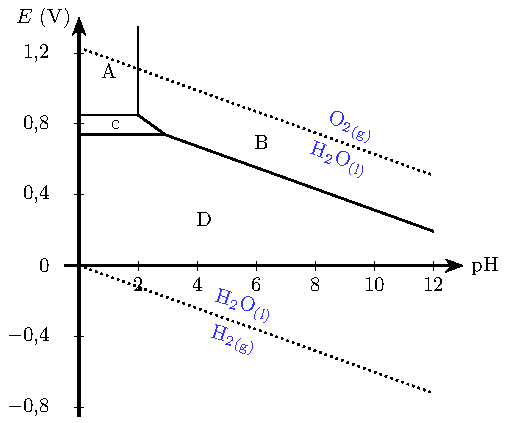
\includegraphics[width=\linewidth]{eph_hg-eau_plain}
		\end{center}
	\end{minipage}
}%

\QR{%
Attribuer un domaine à chaque espèce, en précisant s'il s'agit d'un domaine de
prédominance ou d'existence.
}{%
~
\smallbreak
\vspace*{-25pt}
\noindent
\begin{minipage}[c]{.60\linewidth}
	\begin{center}
		\begin{tabularx}{\linewidth}{YYYYY}
			\toprule
			Espèce                &
			$\ce{Hg_{\liq}}$      &
			$\ce{Hg^2+_{\aqu}}$   &
			$\ce{Hg_2^2+_{\aqu}}$ &
			$\ce{HgO_{\sol}}$
			\\
			\no{Hg}               &
			0                     &
			+\myRoman{2}          &
			+\myRoman{1}          &
			+\myRoman{2}
			\\
			Domaine               &
			D                     & A       & C       & B
			\\
			Type                  &
			Exist.                & Prédom. & Prédom. & Exist.
			\\
			\bottomrule
		\end{tabularx}
	\end{center}
\end{minipage}
\hfill
\begin{minipage}[c]{.39\linewidth}
	\vspace*{0pt}
	\begin{center}
		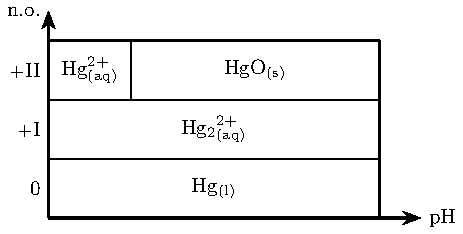
\includegraphics[width=\linewidth]{esit_hg}
	\end{center}
\end{minipage}
\bigbreak
On prouve le caractère acide de \ce{Hg^2+} par une équation~:
\[
	\ce{{Hg}^2+ + H_2O_{\liq} = HgO_{\sol} + 2 {H}^+_{\aqu}}
\]
}%
\QR{%
	Le diagramme $E-\pH$ de l'eau a été tracé en pointillés. Le mercure métal
	est-il stable dans l'eau pure~? dans de l'eau «~aérée~» (c'est-à-dire avec de
	l'oxygène)~? Pour les situations instables, discutez de la nature des espèces
	créées en fonction des conditions du milieu, et écrire les équations
	associées.
}{%
	Dans l'eau sans oxygène, le mercure métal est stable. En revanche, en présence
	de dioxygène il est instable, et pourra former \ce{Hg_2^2+} et \ce{Hg^2+} pour
	un faible pH, ou le solide \ce{HgO} pour $\pH \gtrsim 2$. Les équations
	correspondantes sont~:
	\begin{align*}
		\ce{2Hg_{\liq} + {O_2}_{\gaz} + 4 {H}^+_{\aqu} & = 2 {Hg}^2+_{\aqu}
		+ 2H_2O_{\liq}}
		\\\beforetext{et}
		\ce{2 Hg_{\liq} + {O_2}_{\gaz}                 & = 2HgO_{\sol}}
	\end{align*}
}%
\QR{%
Retrouver la constante de l'équilibre $\ce{{Hg}^2+_{\aqu} + 2
		{HO}^-_{\aqu} = HgO_{\sol} + H_2O_{\liq}}$
}{%
\leavevmode\vspace*{-15pt}\relax
\begin{gather*}
	K = \frac{{c^\circ}^3}{[\ce{Hg}^2+]\ind{eq}[\ce{HO^-}]^2\ind{eq}}
	\\\beforetext{à la frontière}
	\Ra
	\pk[] = \underbracket{\log c_0}_{=0} - 2
	\underbracket{\pOH\ind{front}}_{\pk[e]-\pH\ind{front}}
	\\\Lra
	\boxed{K = 10^{2(\pH\ind{front} - \pk[e])}}
	\Ra
	\xul{K = \num{e-24}}
\end{gather*}
}%
\QR{%
	Calculer la pente de la frontière B/C.
}{%
	\leavevmode\vspace*{-15pt}\relax
	\begin{gather*}
		\beforetext{Couple \ce{HgO/Hg_2^2+}}
		\ce{{Hg_2}^{2+}_{\aqu} + 2H_2O_{\liq} = 2HgO_{\sol} + 4
			{H}^+_{\aqu} + 2e^-}
		\\\Ra
		E = E^\circ(\ce{HgO/Hg_2^{2+}}) + \frac{\num{0.06}}{2} \log
		\frac{[\ce{H^+}]^4}{[\ce{Hg_2^{2+}}]{c^\circ}^3}
		\\\Lra
		E\ind{front} = E^\circ(\ce{HgO/Hg_2^{2+}}) \xul{\num{-0.012}\pH}
	\end{gather*}
}%
\QR{%
	Écrire l'équation bilan de la réaction ayant lieu lorsque l'on augmente le pH
	d'une solution aqueuse contenant l'espèce C. Comment appelle-t-on ce type de
	réaction~?
}{%
	Au-delà de $\pH = 3$, $\ce{Hg_2^2+}$ n'est plus stable et il \textbf{se
		dismute} en $\ce{HgO_{\sol}}$ et $\ce{Hg_{\liq}}$. On écrit les équations
	associées~:
	\begin{align*}
		\beforetext{Couple \ce{Hg_2^2+/Hg}}
		\ce{2 {Hg}_{\liq}                   & = {Hg_2}^2+_{\aqu} + 2e^-}
		\tag{1}
		\\\beforetext{Couple \ce{HgO/Hg_2^2+}}
		\ce{{Hg_2}^2+_{\aqu} + 2 H2O_{\liq} & = 2 HgO_{\sol} + 4 {H}^+ + 2e^-}
		\tag{2}
		\\\beforetext{Réaction}
		\ce{{Hg_2}^2+_{\aqu} + H_2O_{\liq}  & = HgO_{\sol} + Hg_{\liq} + 2
			{H}^+_{\aqu}}
		\tag*{$(3) = (2)-(1)$}
	\end{align*}
}%

\enonce{%
	Lorsque l'on veut tester la présence d'ions mercure en solution aqueuse, on
	peut opérer de la manière suivante~:
	«~\textit{Déposer une goutte de la solution aqueuse acidifiée à tester sur une
		lame de cuivre préalablement polie. Attendre quelques instants et laver la
		lame à l'eau. S'il se forme un amalgame blanc brillant sur la lame de cuivre, la
		solution contient des ions mercure}~».
	\smallbreak
	On indique qu'un amalgame est un alliage de mercure \ce{Hg} et d'un autre métal
	\ce{M}, noté \ce{MHg}. On donne $E^\circ (\ce{Cu^2+ /Cu}) = \SI{0.34}{V}$.
}%
\QR{%
	Pourquoi la solution à tester doit-elle être acidifiée~? Pour quels ions du
	mercure ce protocole est-il valable~? Écrire les équations bilans des
	réactions possibles en milieu acide.
}{%
	\noindent
	\begin{minipage}[t]{.70\linewidth}
		On a déterminé que les ions mercure n'existaient en solution que pour de
		faibles pH~: on acidifie la solution pour éviter la précipitation en \ce{HgO}.
		\bigbreak
		Grâce à une échelle en $E^\circ$, on voit que ce protocole est valable pour
		\textbf{les deux ions du mercure}. Les équations associées sont~:
		\begin{gather*}
			\ce{{Hg_2}^2+_{\aqu} + Cu_{\sol} = 2 Hg_{\liq} + {Cu}^2+_{\aqu}}
			\\\beforetext{et}
			\ce{2 {Hg}^2+_{\aqu} + 2 Cu_{\sol} = 2Hg_{\liq} + 2 {Cu}^2+_{\aqu}}
		\end{gather*}
	\end{minipage}
	\hfill
	\begin{minipage}[t]{.27\linewidth}
		\vspace{0pt}
		\begin{center}
			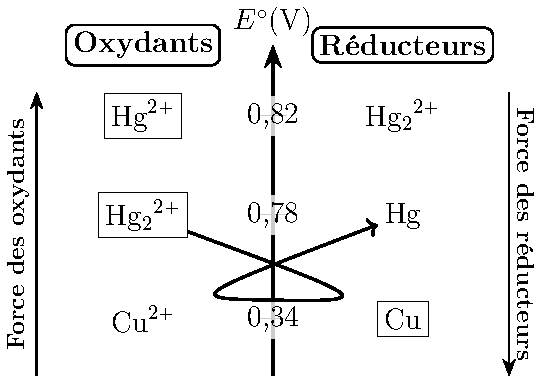
\includegraphics[width=\linewidth]{estand_amalgcu}
		\end{center}
	\end{minipage}
}%

\resetQ
\section{Eau de Javel}
\enonce{%
	On dit souvent qu'il ne faut pas mélanger les produits ménagers, en
	particulier l'eau de Javel et un acide. Essayons de comprendre pourquoi.
	\smallbreak
	\noindent
	\begin{minipage}[c]{.55\linewidth}
		Le dichlore est un gaz toxique irritant, pouvant entraîner de graves problèmes
		pulmonaires en cas d'inhalation. Une solution aqueuse de dichlore
		$\ce{{Cl_2}_{\aqu}}$ peut libérer du dichlore gazeux
		$\ce{{Cl_2}_{\gaz}}$. L'eau de Javel est une solution aqueuse comportant du
		chlorure de sodium $(\ce{{Na}^+_{\aqu}};\ce{{Cl}^-}_{\aqu})$ et de
		l'hypochlorite de sodium $(\ce{{Na}^+_{\aqu}};\ce{{ClO}^-_{\aqu}})$ en
		quantité équimolaire.
		\smallbreak
		Le diagramme potentiel-pH simplifié de l'élément chlore est représenté
		ci-contre, pour les espèces chimiques $\ce{HClO_{\aqu}}$,
		$\ce{{ClO}^-_{\aqu}}$, $\ce{{Cl_2}_{\aqu}}$ et $\ce{{Cl}^-_{\aqu}}$.
		La convention de tracé est fixée à $c_t = \SI{0.1}{mol.L^{-1}}$.
	\end{minipage}
	\hfill
	\begin{minipage}[c]{.45\linewidth}
		\vspace{0pt}
		\begin{center}
			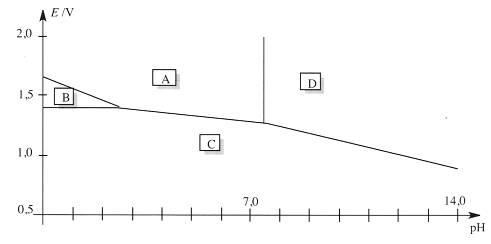
\includegraphics[width=\linewidth]{eph_javel-moche_white}
		\end{center}
	\end{minipage}
	\begin{tcb}(data)<lfnt>{Données}
		À \SI{298}{K} et $\pH = 0$, $E^\circ (\ce{HClO_{\aqu}/{Cl_2}_{\aqu}})
			= \SI{1.60}{V}$ et $E^\circ (\ce{{Cl_2}_{\aqu}/{Cl}^-_{\aqu}}) =
			\SI{1.39}{V}$.
	\end{tcb}
}%

\QR{%
Indiquer les espèces chimiques auxquelles correspondent les domaines notés A,
B, C et D.
}{%
~
\smallbreak
\vspace*{-25pt}
\noindent
\begin{minipage}[c]{.60\linewidth}
	\begin{center}
		\begin{tabularx}{\linewidth}{YYYYY}
			\toprule
			Espèce                &
			$\ce{HClO_{\aqu}}$    &
			$\ce{{ClO}^-_{\aqu}}$ &
			$\ce{{Cl_2}_{\aqu}}$  &
			$\ce{{Cl}^-_{\aqu}}$
			\\
			\no{Cl}               &
			+\myRoman{1}          &
			+\myRoman{1}          &
			0                     &
			-\myRoman{1}
			\\
			Domaine               &
			A                     & D & B & C
			\\
			\bottomrule
		\end{tabularx}
	\end{center}
\end{minipage}
\hfill
\begin{minipage}[c]{.39\linewidth}
	\vspace*{0pt}
	\begin{center}
		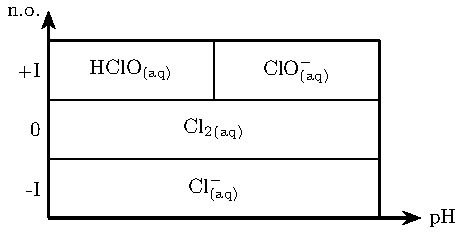
\includegraphics[width=\linewidth]{esit_chlore}
	\end{center}
\end{minipage}
\smallbreak
On prouve le caractère acide de \ce{HClO} par une équation~:
\[
	\ce{HClO_{\aqu} + H_2O_{\liq} = {ClO}^-_{\aqu} + {H_3O}^+_{\aqu}}
	\tag*{$K_A$}
\]
}%
\QR{%
Retrouver graphiquement la valeur du $\pk$ du couple acido-basique
$\ce{HClO_{\aqu}/{ClO}^-_{\aqu}}$.
}{%
Pour des espèces acido-basiques dissoutes, par la relation de \textsc{Henderson}
on a
\[
	\boxed{\pH\ind{front} = \pk}
	\Ra
	\xul{\pk = \num{7.25}}
\]
}%
\QR{%
	En utilisant le diagramme $E-\pH$, prévoir l'évolution d'un mélange contenant
	les espèces A et C lors du passage en milieu très acide $(\pH < \num{2.5})$.
	Écrire alors l'équation bilan de la réaction correspondante. Comment s'appelle
	une telle réaction~? Calculer sa constante d'équilibre à \SI{298}{K}.
}{%
	\noindent
	\begin{minipage}[t]{.80\linewidth}
		À faible pH, le \ce{HClO} et les ions \ce{Cl^-} auront des domaines
		disjoints~: ils vont réagir ensemble pour \textbf{former du \ce{Cl2}}. C'est
		une \textbf{médiamutation}, qu'on peut représenter par le diagramme en
		$E^\circ$ ci-contre.
		\begin{align*}
			\beforetext{Couple $\ce{HClO_{\aqu}/{Cl_2}_{\aqu}}$}
			\hspace{80pt}
			\ce{{Cl_2}_{\aqu} + 2H_2O_{\liq} & = 2HClO_{\aqu} + 2 {H}^+_{\aqu} + 2e^-}
			\tag{1}
			\\\beforetext{Couple $\ce{{Cl_2}_{\aqu}/{Cl}^-_{\aqu}}$}
			\ce{2 {Cl}^-_{\aqu}              & = {Cl_2}_{\aqu} + 2e^-}
			\tag{2}
		\end{align*}
	\end{minipage}
	\hfill
	\begin{minipage}[t]{.20\linewidth}
		\vspace{0pt}
		\begin{center}
			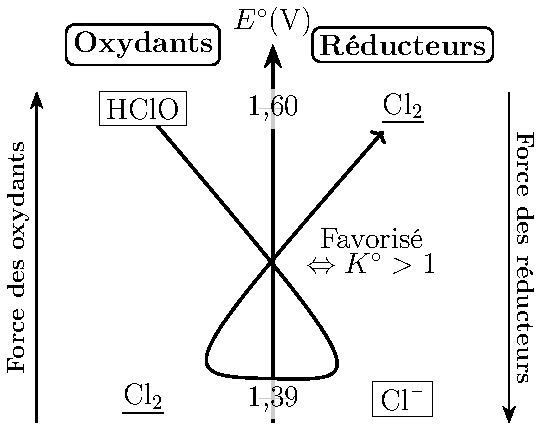
\includegraphics[width=\linewidth]{estand_mediamut_cl2}
		\end{center}
	\end{minipage}
	\hspace*{\fill}
	\begin{gather*}
		\beforetext{Réaction}
		\ce{HClO_{\aqu} + {H}^+_{\aqu} + {Cl}^-_{\aqu} = {Cl_2}_{\aqu} +
		H2O_{\liq}}
		\tag*{$(3) = [(2)-(1)]/2$}
		\\
		\beforetext{Couple $\ce{HClO_{\aqu}/{Cl_2}_{\aqu}}$}
		E_1 = E^\circ(\ce{HClO/Cl_2}) + \frac{\num{0.06}}{2} \log
		(\frac{p_{\ce{Cl_2}}{c^\circ}^4}{p^\circ [\ce{HClO}]^2 [\ce{H^+}]^2})
		\\
		\beforetext{Couple $\ce{{Cl_2}_{\aqu}/{Cl}^-_{\aqu}}$}
		E_2 = E_2^\circ (\ce{{Cl_2}_{\aqu}/{Cl}^-_{\aqu}}) +
		\frac{\num{0.06}}{2} \log (\frac{p^\circ [\ce{Cl^-}]^2}{p_{\ce{Cl_2}}})
		\\
		\beforetext{$E_1 = E_2 \Lra$}
		E_1^\circ - E_2^\circ = \frac{\num{0.06}}{2} \log
		\underbracket{\left(\frac{p_{\ce{Cl_2}}^2 {c^\circ}^6}
			{{p^\circ}^2[\ce{HClO}]^2 [\ce{H^+}]^2 [\ce{Cl^-}]^2}\right)}_{K^2}
		\\
		\Lra
		\boxed{K = 10^{\DS \frac{1}{\num{0.06}}(E_1^\circ - E_2^\circ)}}
		\Ra
		\xul{K^\circ = 10^{\num{3.50}}}
	\end{gather*}
	Elle est donc totale. On fait attention au nombre totale d'électrons échangés,
	ici avec le choix de nombres stœchiométriques on a bien 1 seul électron
	échangé.
}%
\QR{%
	Lorsque $\ce{{Cl_2}_{\aqu}}$ se forme au sein de la solution, un équilibre
	s'établit alors avec $\ce{{Cl_2}_{\gaz}}$, ce qui entraîne un dégagement
	gazeux. Pourquoi ne faut-il donc jamais mélanger l'eau de Javel avec un
	acide~?
}{%
	On voit que \ce{ClO^-} en milieu acide donne \ce{HClO}, et on vient de
	démontrer qu'en milieu très acide \ce{HClO} et \ce{Cl^-} formaient du
	$\ce{{Cl_2}_{\aqu}}$, donnant lui-même du dichlore gazeux très toxique~!
}%

\resetQ
\section{Autour du chrome}
\subsection{Diagramme $E-\pH$ du chrome}
\enonce{%
On donne le diagramme $E-\pH$ du chrome auquel se superpose celui de l'eau. On
étudie $\ce{{Cr}^2+_{\aqu}}$, $\ce{{CrO_4}^2-_{\aqu}}$,
$\ce{{CrO_2}^-_{\aqu}}$, $\ce{{Cr}^3+_{\aqu}}$,
$\ce{{Cr_2O_7}^2-_{\aqu}}$, $\ce{Cr_{\sol}}$ et
$\ce{{Cr(OH)_3}_{\sol}}$. On donne $E^\circ (\ce{Cr^2+ /Cr}) =
	\SI{-0.91}{V}$.
}%
\QR{%
Dans cette question, on ne prend en compte que les espèces
$\ce{{Cr}^2+_{\aqu}}$, $\ce{{CrO_2}^-_{\aqu}}$,
$\ce{{Cr}^3+_{\aqu}}$, $\ce{Cr_{\sol}}$ et $\ce{{Cr(OH)_3}_{\sol}}$.
Indiquer pour chacun des domaines numérotés de 1 à 5 sur le diagramme à quelle
espèce chimique il correspond, ainsi que la nature du domaine.
}{%
~
\smallbreak
\vspace*{-25pt}
\noindent
\begin{minipage}[c]{.60\linewidth}
	\begin{center}
		\begin{tabularx}{\linewidth}{YYYYYY}
			\toprule
			Espèce                  &
			$\ce{Cr_{\sol}}$        &
			$\ce{Cr^2+_{\aqu}}$     &
			$\ce{{Cr}^{3+}_{\aqu}}$ &
			$\ce{{Cr(OH)_3}_{\sol}}$
			$\ce{{CrO_2}^-_{\sol}}$
			\\
			\no{Cr}                 &
			0                       &
			+\myRoman{2}            &
			+\myRoman{3}            &
			+\myRoman{3}            &
			+\myRoman{3}
			\\
			Domaine                 &
			\circled{1}             & \circled{2} & \circled{5} & \circled{3} & \circled{4}
			\\
			\bottomrule
		\end{tabularx}
	\end{center}
\end{minipage}
\hfill
\begin{minipage}[c]{.39\linewidth}
	\vspace*{0pt}
	\begin{center}
		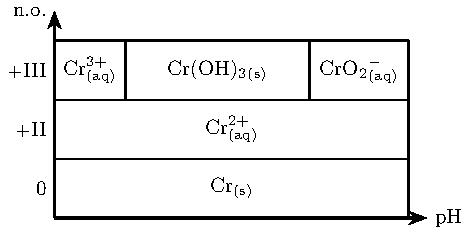
\includegraphics[width=\linewidth]{esit_cr}
	\end{center}
\end{minipage}
\bigbreak
On prouve le comportement acido-basique des éléments de $\no{Cr} = +\myRoman{3}$
par les équations~:
\begin{gather*}
	\beforetext{Couple \ce{Cr^{3+}/Cr(OH)_3}~:}
	\ce{{Cr}^{3+}_{\aqu} + 3 {HO}^-_{\aqu} = {Cr(OH)_3}_{\sol} + H_2O_{\liq}}
	\tag*{$K_{A,1} = \frac{1}{K_s}$}
	\\
	\beforetext{Couple \ce{Cr(OH)_{3}/CrO_2^-}~:}
	\ce{{Cr(OH)_3}_{\sol} = {CrO_2}^{-}_{\aqu} + {H_3O}^{+}_{\aqu}}
	\tag*{$K_{A,2}$}
\end{gather*}
}%
\QR{%
	Déduire par lecture du diagramme la valeur de la concentration de tracé $c_t$,
	concentration de chaque espèce dissoute contenant l'élément chrome à la
	frontière.
}{%
	Grâce au couple $\ce{Cr^{2+}/Cr}$, on a
	\begin{gather*}
		E\ind{front} = E^\circ + \frac{\num{0.06}}{2} \log c_t
		\qav
		\left\{
		\begin{array}{rcl}
			E\ind{front} & = & \SI{-0.91}{V}
			\\
			E^\circ      & = & \SI{-0.91}{V}
		\end{array}
		\right.\\
		\AN
		\xul{
			c_t = \SI{1.0}{mol.L^{-1}}
		}
	\end{gather*}
}%
\QR{%
	Déduire du diagramme le $\pk[s]$ de $\ce{{Cr(OH)_3}_{\sol}}$ ainsi que la
	constante de la réaction de dissolution de $\ce{{Cr(OH)_3}_{\sol}}$ en
	milieu basique.
}{%
	\leavevmode\vspace*{-15pt}\relax
	\begin{gather*}
		K_s = \frac{c_t [\ce{HO^-}]\ind{front}^3}{{c^\circ}^4}
		\Lra
		\pk[s] = 0 + 3 \pOH\ind{front} = 3(\pk[e] - \pH\ind{front})
		\Ra
		\xul{\pk[s] = 30}
		\\\beforetext{En milieu basique,}
		\ce{{Cr(OH)_3}_{\sol} + {HO}^-_{\aqu} = {CrO_2}^-aqu + 2 H_2O_{\liq}}
		\tag*{$K\ind{dis}$}
		\\\Lra
		K\ind{dis} = \frac{c_t}{[\ce{HO^-}]\ind{front}}
		\Lra
		\pk[\rm dis] = -\pOH\ind{front} = \pH\ind{front} - \pk[e]
		\\\Lra
		\xul{\pk[\rm dis] = \num{10.4}}
	\end{gather*}
}%
\QR{%
On souhaite compléter le diagramme $E-\pH$ du chrome en prenant en compte, en
plus des espèces précédentes, les ions chromates $\ce{{CrO_4}^2-_{\aqu}}$
et dichromates $\ce{{Cr_2O_7}^2-_{\aqu}}$. Indiquer à quelle espèce
chimique correspond chacun des domaines numérotés 6 et 7.
}{%
On pourrait calculer le \no{Cr} dans ces composés, mais forcément ils sont soit
\circled{6} soit \circle{7} (sinon c'est +\myRoman{6}). Or ces deux domaines
sont séparés par une frontière verticale, ce sont donc les espèces d'un couple
acide-base. On l'équilibre pour trouver~:
\[
	\underbracket[1pt]{\ce{{Cr_2O_7}^{2-}_{\aqu}}}_{\text{diacide}}
	\ce{+ H_2O_{\liq} =}
	\underbracket[1pt]{\ce{2 {CrO_4}^{2-}}}_{\text{base}}
	\ce{+ 2 {H}^+_{\aqu}}
\]
Ainsi, \circled{6} est $\ce{Cr_2O_7^2-}$ et \circled{7} est $\ce{CrO_4^2-}$.
}%

\enonce{%
	\begin{center}
		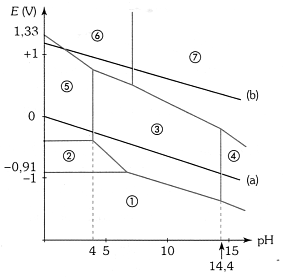
\includegraphics[width=.5\linewidth]{eph_cr-moche_white}
	\end{center}
}%

\subsection{Étude de réactions du chrome et de ses composés}
\begin{blocQR}
	\item \enonce{%
		Sur le diagramme précédent, on a également porté les droites délimitant le
		domaine de stabilité thermodynamique de l'eau.
	}%
	\QR{%
		Quels sont les composés du chrome au degré d'oxydation +\myRoman{6} qui sont
		stables en solution aqueuse~? Pour ceux qui seraient instables, on donnera
		l'équation de la réaction à laquelle ils donnent lieu.
	}{%
		Les ions $\ce{{CrO_4}^{2-}_{\aqu}}$ ont un domaine joint avec l'eau~: ils
		sont \textbf{stables} dans l'eau désaérée. Les ions
		$\ce{{Cr_2O_7}^{2-}_{\aqu}}$ le sont également à condition que le pH ne soit
		pas trop faible. Sinon on a une réaction avec l'eau telle que~:
		\begin{align*}
			\beforetext{$\ce{{Cr_2O_7}^{2-}/Cr^{3+}}$}
			\ce{2 {Cr}^{3+}_{\aqu} + 7 H_2O_{\liq}     & = {Cr_2O_7}^{2-}_{\aqu} + 6 e^- +
			14 {H}^+_{\aqu}}
			\tag{1}
			\\
			\beforetext{\ce{O_2/H_2O}}
			\ce{
			H_2O_{\liq}                                & = \frac{1}{2} {O_2}_{\gaz} + 2 {H}^+_{\aqu} + 2 e^-
			}
			\tag{2}
			\\
			\ce{{Cr_2O_7}^{2-}_{\aqu} + 8 {H}^+_{\aqu} & = 2 {Cr}^{3+} + \frac{3}{2}
			{O_2}_{\gaz} + 4H_2O_{\liq}}
			\tag*{$(3) = 3(2) - (1)$}
		\end{align*}
		En réalité, les surtensions cinétiques (cf.\ année prochaine) rendent cette
		réaction infiniment lente~: on utilise couramment des solutions de
		dichromate en milieu acide sulfurique en laboratoire.
	}%
	\QR{%
	Les ions $\ce{{Cr}^3+_{\aqu}}$ sont-ils stables en solution aqueuse~?
	Quelle(s) réaction(s) peuvent-ils donner avec l'eau~?
	}{%
	Les ions \ce{Cr^3+} sont stables dans l'eau du point de vue redox par domaine
	joint~; par contre ils précipitent dans l'eau pure sous la forme
	$\ce{{Cr(OH)_3}_{\sol}}$.
	}%
	\item \enonce{%
	On étudie l'action du dichromate sur le fer II, en milieu de $\pH < 6$. Dans
	ces conditions, les potentiels des couples sont~:
	\begin{itemize}
		\item $\pH < \num{1.33}$~:
		      $E^\circ(\ce{{Fe}^3+_{\aqu}/{Fe}^2+_{\aqu}}) = \SI{0.77}{V}$~;
		\item $\num{1.33} < \pH < \num{6.5}$~: $E^\circ
			      (\ce{{Fe(OH)_3}_{\sol}/{Fe}^3+}_{\aqu}) = \num{1.01} -
			      \num{0.18}\pH$ (en volts).
	\end{itemize}
	\resetQ
	\QR{%
	Quels sont les produits obtenus par l'action du dichromate sur le fer II
	en milieu de $\pH < 6$~?
	}{%
	$\ce{Cr_2O_7^{2-}}$ oxyde le fer II en fer III car leurs domaines de
	prédominance sont disjoints pour tout pH~:
	\begin{itemize}
		\item $\num{0.00} < \pH < \num{1.33}$~: on obtient \ce{Fe^3+} et \ce{Cr^3+}~;
		\item $\num{1.33} < \pH < \num{4.00}$~: on obtient \ce{Fe(OH)_3} et
		      \ce{Cr^3+}~;
		\item $\num{4.00} < \pH < \num{6.00}$~: on obtient \ce{Fe(OH)_3} et
		      \ce{Cr(OH)_3}.
	\end{itemize}
	}%
	\begin{blocQR}
		\item \enonce{%
			On opère en général à pH voisin de 0.
		}%
		\QR{%
			Écrire l'équation de la réaction dans ce cas. Est-elle totale~?
		}{%
			\leavevmode\vspace*{-15pt}\relax
			\begin{gather*}
				\ce{{Cr_2O_7}^{2-}_{\aqu} + 6 {Fe}^{2+}_{\aqu} + 14 {H}^+_{\aqu} ->
				2 {Cr}^{3+}_{\aqu} + 6 {Fe}^{3+}_{\aqu} + 7H_2O_{\liq}}
				\\
				\boxed{K^\circ = 10^{\DS \frac{E^\circ(\ce{Cr_2O_7^{2-}/Cr^{3+}}) -
								E^\circ (\ce{Fe^{3+}/Fe^{2+}})}{\num{0.01}}}}
				\Ra
				\xul{K^\circ = \num{e56}}
			\end{gather*}
			La réaction est donc effectivement totale.
		}%
		\QR{%
			Commenter le choix du pH.
		}{%
			C'est à $\pH = 0$ que le dichromate est le plus oxydant, et à ce pH les
			ions fer II et fer III sont solubles dans l'eau.
		}%
		\QR{%
			L'utilisation du dichromate dans ces conditions est-elle en contradiction
			avec les résultats obtenus aux questions précédentes~?
		}{%
			Nous avons vu que $\ce{Cr_2O_7^2-}$ était instable thermodynamiquement à
			pH nul, mais \textit{métastable} cinétiquement.
		}%
	\end{blocQR}
	}%
\end{blocQR}

\resetQ
\section{Dosage du glucose}
\enonce{%
	\noindent
	\begin{minipage}[c]{.55\linewidth}
		On donne l'allure du diagramme $E-\pH$ relatif aux substances iodées. On se
		limite aux espèces suivantes~: le diiode $\ce{{I_2}_{\aqu}}$, les ions
		iodate $\ce{{IO_3}^-_{\aqu}}$ et les ions iodure $\ce{{I}^-_{\aqu}}$. La
		concentration de chacune des espèces iodées est égale à $c_t =
			\SI{0.10}{mol.L^{-1}}$ sur les frontières.
		\smallbreak
		On indique que le $\ce{{I_2}_{\aqu}}$ a une coloration brune en solution,
		les autres espèces iodées sont incolores.
		\smallbreak
		On s'intéresser à un protocole permettant de déterminer la quantité de
		glucose dans une cannette de \textit{Redbull}. On détaille ci-dessous le
		protocole expérimental du dosage~:
	\end{minipage}
	\hfill
	\begin{minipage}[c]{.45\linewidth}
		\vspace{0pt}
		\begin{center}
			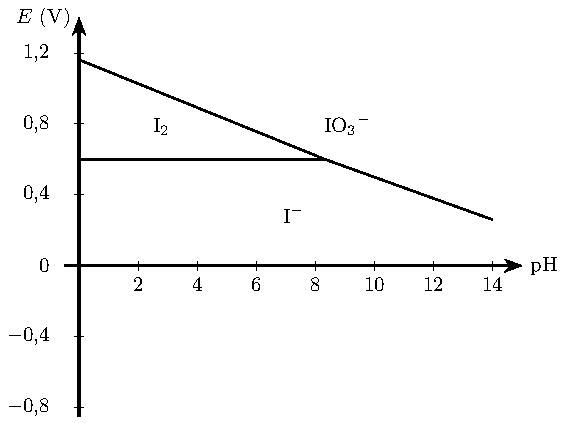
\includegraphics[width=\linewidth]{eph_iode}
		\end{center}
	\end{minipage}

	\begin{enumerate}[label=\clenumi]
		\item On introduit dans un erlenmeyer un volume $V_1 = \SI{20.0}{mL}$ d'une
		      solution de diiode de concentration $c_1 = \SI{0.050}{mol.L^{-1}}$~;
		\item On ajoute dans l'erlenmeyer $\SI{5}{mL}$ d'une solution d'hydroxyde de
		      sodium $(\ce{{Na}^+_{\aqu}};\ce{{HO}^-_{\aqu}})$ à
		      \SI{2.5}{mol.L^{-1}}. La solution se décolore.
		\item On ajoute au mélange précédent un volume $V_0 = \SI{2.0}{mL}$ de
		      \textit{Redbull}, de concentration en glucose $c_0$ inconnue. On
		      bouche l'erlenmeyer, on l'agite et on laisse agir 30 minutes dans
		      l'obscurité.
		\item Après cette attente, on ajoute dans l'erlenmeyer $\SI{10}{mL}$ d'acide
		      chlorhydrique $(\ce{{H}^+_{\aqu}};\ce{{Cl}^-_{\aqu}})$ à
		      \SI{2}{mol.L^{-1}}. La coloration brune réapparait.
		\item Une solution de thiosulfate de sodium
		      $(\ce{2{Na}^+_{\aqu}};\ce{{S_2O_3}^2-_{\aqu}})$ de concentration
		      $c_2 = \SI{0.10}{mol.L^{-1}}$ est introduite dans une burette. On
		      titre le contenu de l'erlenmeyer en présence d'empois d'amidon. On
		      observe alors une décoloration complète de la solution pour un volume
		      verse de thiosulfate de sodium noté $V\ind{2,eqv}$.
	\end{enumerate}
}%

\QR{%
À la lumière du diagramme $E-\pH$ de l'iode, quelle réaction s'est produite
lors de l'étape \circled{2}~? Écrire l'équation de cette réaction et nommer de
type de réaction.
}{%
En milieu basique, le diiode est instable et se dismute en ions iodure et en
ions iodate. Le bilan est écrit en combinant les deux demi-équations
relatives aux couples $\ce{{IO_3}^{-}_{\aqu}/{I_2}_{\aqu}}$ et
$\ce{{I_2}_{\aqu}/{I}^-_{\aqu}}$, et en tenant compte de la basicité du milieu
(i.e.\ on fait disparaître les ions \ce{H^+} présents dans le bilan en les
combinant avec des ions hydroxyde sous forme de molécules d'eau). Le résultat
obtenu est une réaction de \textbf{dismutation}~:
\[
	\ce{3 {I_2}_{\aqu} + 6 {HO}^-_{\aqu} = 3 H_2O_{\liq} + 5 {I}^-_{\aqu} +
	{IO_3}^-_{\aqu}}
\]
}%
\QR{%
Lors de l'étape \circled{3}, le glucose $\ce{{C_6H_{12}O_6}_{\aqu}}$ est
oxydé en ions gluconates $\ce{{C_6H_{11}O_7}^-_{\aqu}}$ par les ions iodates
en milieu basique. Écrire la réaction bilan qui se produit pendant cette
étape.
}{%
Le bilan est écrit en combinant les demi-équations relatives aux couples
\ce{IO3^{-}/I^-} et $\ce{{C_6H_{11}O_7}^-_{\aqu}/{C_6H_{12}O_6}_{\aqu}}$ en
milieu basique~:
\[
	\ce{3 {C_6H_{12}O_6}_{\aqu} + {IO_3}^{-}_{\aqu} + 3 {HO}^-_{\aqu} =
	3 {C_6H_{11}O_7}^-_{\aqu} + {I}^-_{\aqu} + 3 H_2O_{\liq}}
\]
}%
\QR{%
	À la lumière du diagramme $E-\pH$ de l'iode, quelle réaction s'est produite
	lors de l'étape \circled{4}~? Écrire l'équation de cette réaction et nommer de
	type de réaction.
}{%
	Le passage en milieu acide permet aux ions iodate en excès de réagir avec les
	ions iodure présents de façon à former du diiode (réaction de médiamutation,
	inverse la réaction écrite à la question 1).
}%
\QR{%
Écrire l'équation de la réaction de titrage correspondant à l'étape
\circled{5}. On indique que $E^\circ (\ce{{S_4O_6}^2-/{S_2O_3}^2-}) =
	\SI{0.09}{V}$ et $E^\circ (\ce{I_2/I^-}) = \SI{0.62}{V}$.
}{%
Le diiode formé est ensuite titré par les ions thiosulfate. Le bilan s'écrit~:
\[
	\ce{2 {S_2O_3}^{2-}_{\aqu} + {I_2}_{\aqu} = {S_4O_6}^{2-}_{\aqu} + 2 {I}^-_{\aqu}}
\]
}%
\enonce{%
	Après avoir répété ce protocole trois fois, l'expérimentatrice mesure un
	volume moyen $V\ind{2,eqv} = \SI{15.4}{mL}$.
}%
\QR{%
	Exprimer littéralement, en fonction de $c_1$, $V_1$, $c_2$ et $V\ind{2,eqv}$
	la quantité d'ions iodates $n_3$ ayant réagi avec le glucose (étape
	\circled{3}). En supposant cette réaction totale, et en considérant que le
	glucose est le réactif limitant de cette réaction, en déduire la quantité de
	glucose $n_0$ ayant réagi. Calculer numériquement $c_0$.
}{%
	La quantité de diiode titré à l'étape \circled{5} est égale à~:
	\[
		n (\ce{I_2}) = \frac{c_2V_2}{2}
	\]
	Ce diiode provenait des ions iodate qui n'avaient pas réagi avec le glucose.
	La quantité d'ions iodate qui n'avaient pas réagi est ainsi donnée par
	$\frac{c_2v_2}{6}$. La quantité $n_3$ d'ions iodate ayant réagi avec le
	glucose s'écrit~:
	\[
		n_3 = \frac{c_1V_1}{3} - \frac{c_2V_2}{6}
	\]
	D'où la quantité de glucose dosé est égale à
	\[
		n_0 = c_0V_0 = 3n_3
		\Lra
		\boxed{n_0 = c_1V_1 - \frac{c_2V_2}{2}}
		\Ra
		\xul{c_0 = \SI{0.115}{mol.L^{-1}}}
	\]
}%
\QR{%
	Déduire de la question précédente la masse de glucose présente dans une
	canette de \textit{Redbull} de volume $V = \SI{250}{mL}$. La masse molaire du
	glucose est de $\SI{180}{g.mol^{-1}}$.
}{%
	\leavevmode\vspace*{-15pt}\relax
	\[
		\boxed{m = c_0VM}
		\Ra
		\xul{m = \SI{5.18}{g}}
	\]
	L'OMS recommande \SI{25}{g} de sucre par jour.
}%

\end{document}
